\documentclass[../../../main]{subfiles}
\begin{document}
\section{原理}\label{sec:principle}

\subsection{サーボ機構の基本的動作原理}

サーボ機構とは、物体の位置・方位・姿勢などを指定し、それを維持するための自動制御装置のことである。
これをブロック線図で表すと、図\ref{fig:servo-block-line}のようになる。
\begin{figure}
    \centering
    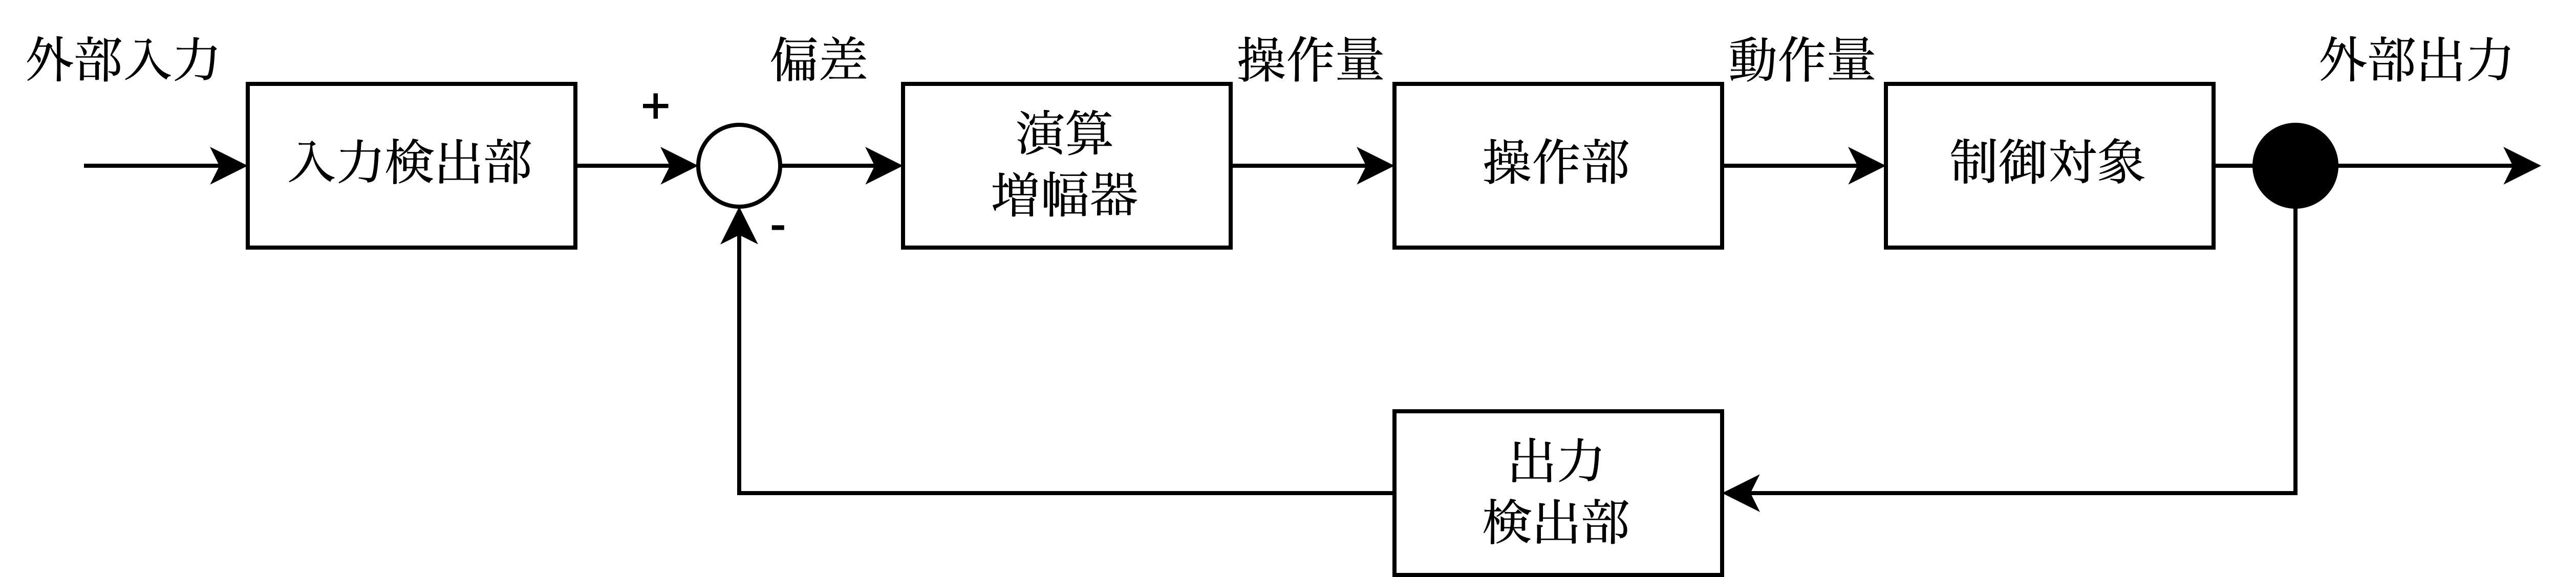
\includegraphics[width=0.8\linewidth]{src/figures/servo-block-line/servo-block-line.png}
    \caption{サーボ機構のブロック線図}\label{fig:servo-block-line}
\end{figure}

本実験では、回転する物体の回転角を制御するための電気式サーボ機構を構築し、その制御を行う。
回転角を制御するための簡単な電動式サーボ機構の図をつくると、図\ref{fig:electric-servo-mechanism}のようになる。
\begin{figure}
	\centering
	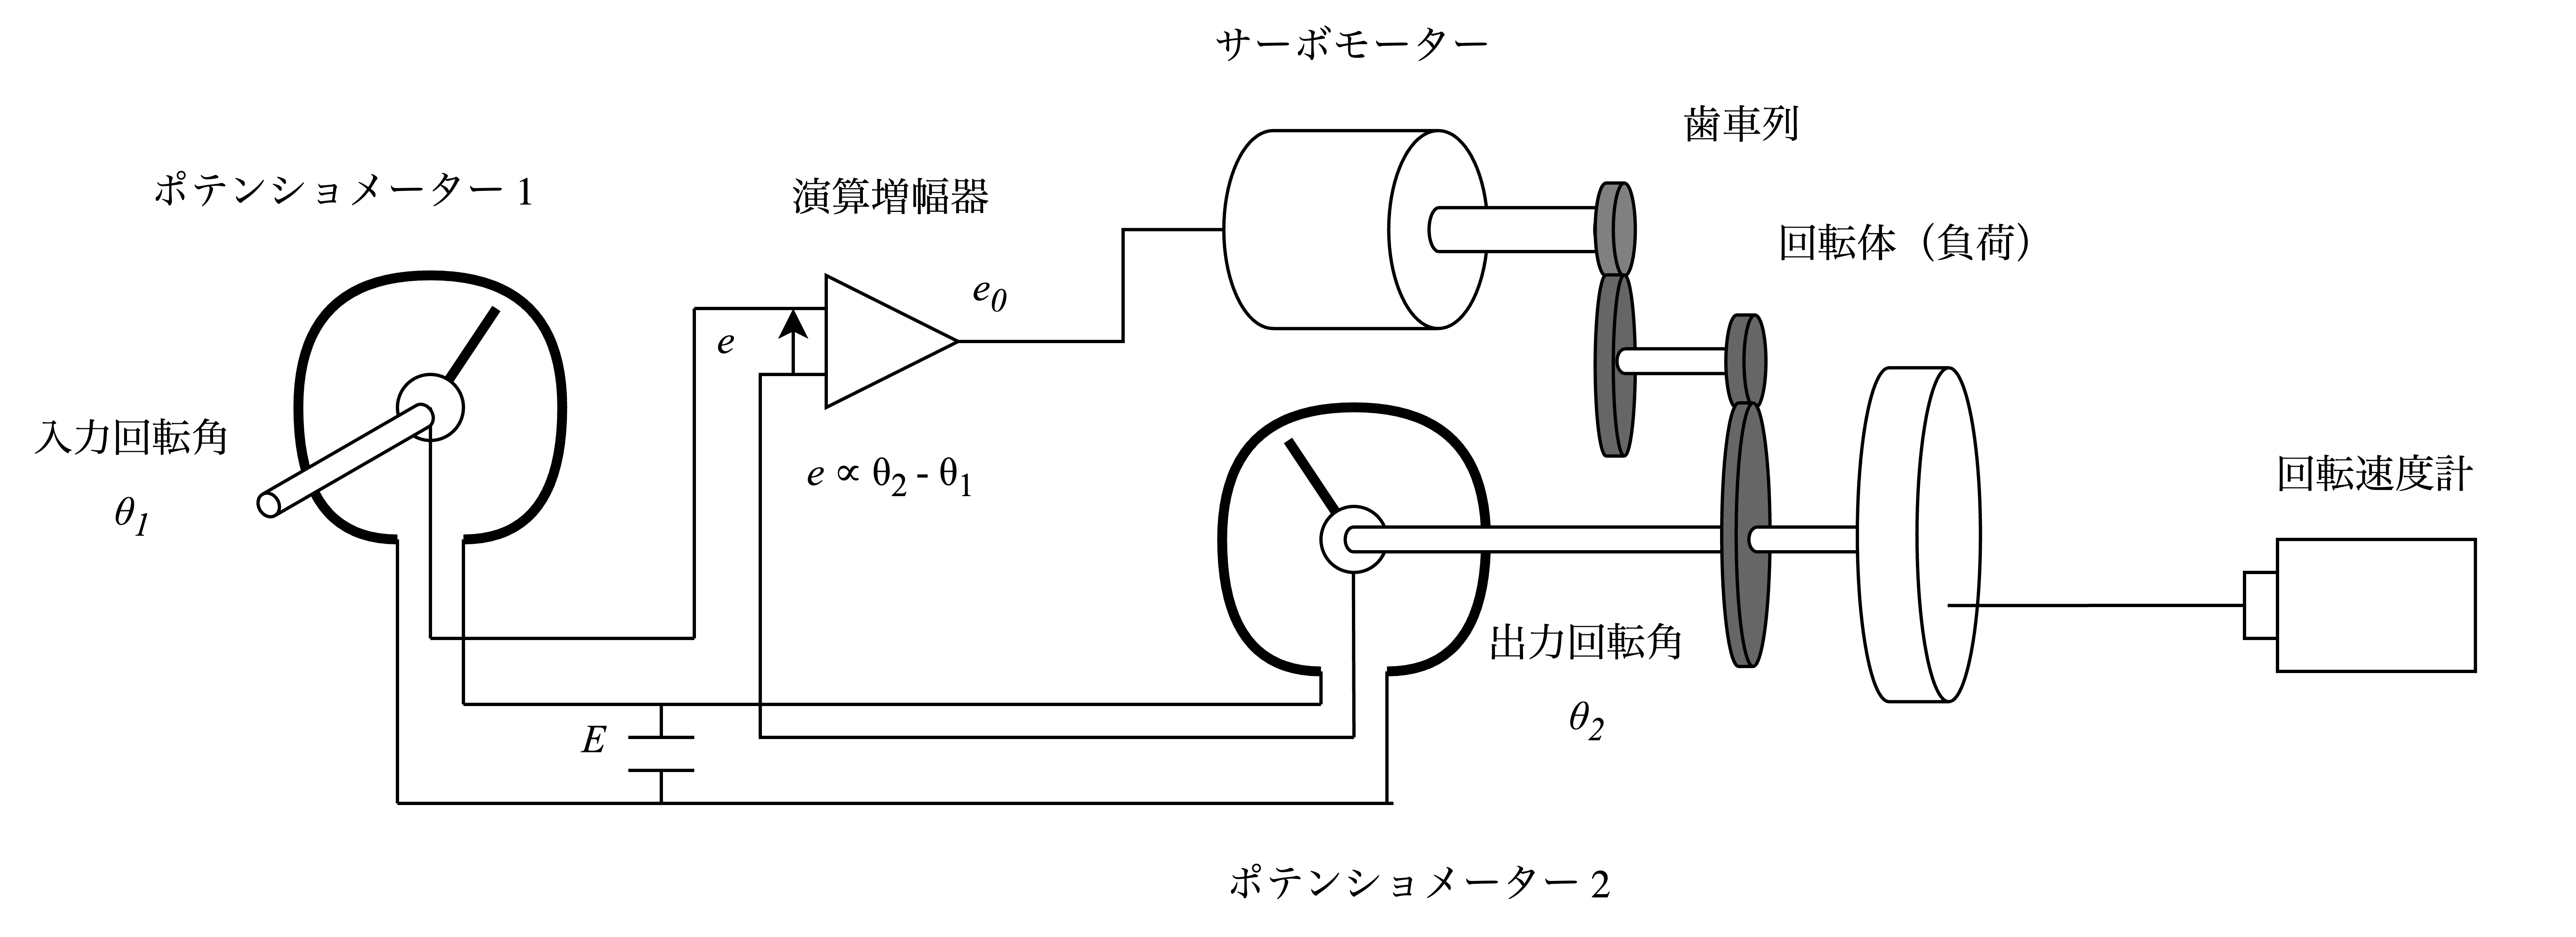
\includegraphics[width=\linewidth]{src/figures/electric-servo-mechanism/electric-servo-mechanism.png}
	\caption{回転角を制御するための電動式サーボ機構の図}\label{fig:electric-servo-mechanism}
\end{figure}

この図\ref{fig:electric-servo-mechanism}において、各要素の対応を表\ref{tab:electric-servo-mechanism-parts}に示す。
\begin{table}[h]
    \centering
    \caption{各要素の対応}\label{tab:electric-servo-mechanism-parts}
    \begin{tabular}{|l|l|}
        \hline
        入力検出結果 & ボディションメーターI    \\
        出力検出結果 & ボディションメーターII   \\
        適合検出結果 & 適合検出器          \\
        投影結果   & サージェントメーター・高度制 \\
        制御対象結果 & 回転機体(全般)       \\
        \hline
    \end{tabular}
\end{table}



\subsection{ポテンショメーターの原理}
入力角度と出力角度を検出するための可変抵抗器の一種である。
ブラシが回転し得る全有効回転角度を$\Theta$、
抵抗線の両端に印加する電圧を$E$とすると、
回転軸からの入力角度$\theta$に対して、
ポテンショメーターから出力する電圧$e$は、
\begin{equation}\label{eq:potentiometer}
    e = E \frac{\theta}{\Theta}
\end{equation}
となる。
入力・出力の2台のポテンショメーターからの電圧による偏差電圧$e$
は次の図\ref{fig:potentio-meter-detection}のように接続することで、
\begin{equation}
    e = \dfrac{E}{\Theta} (\theta_1 - \theta_2)
\end{equation}
として得られ、
入力軸と出力軸の差に応じた電圧が得られる。
\begin{figure}
    \centering
    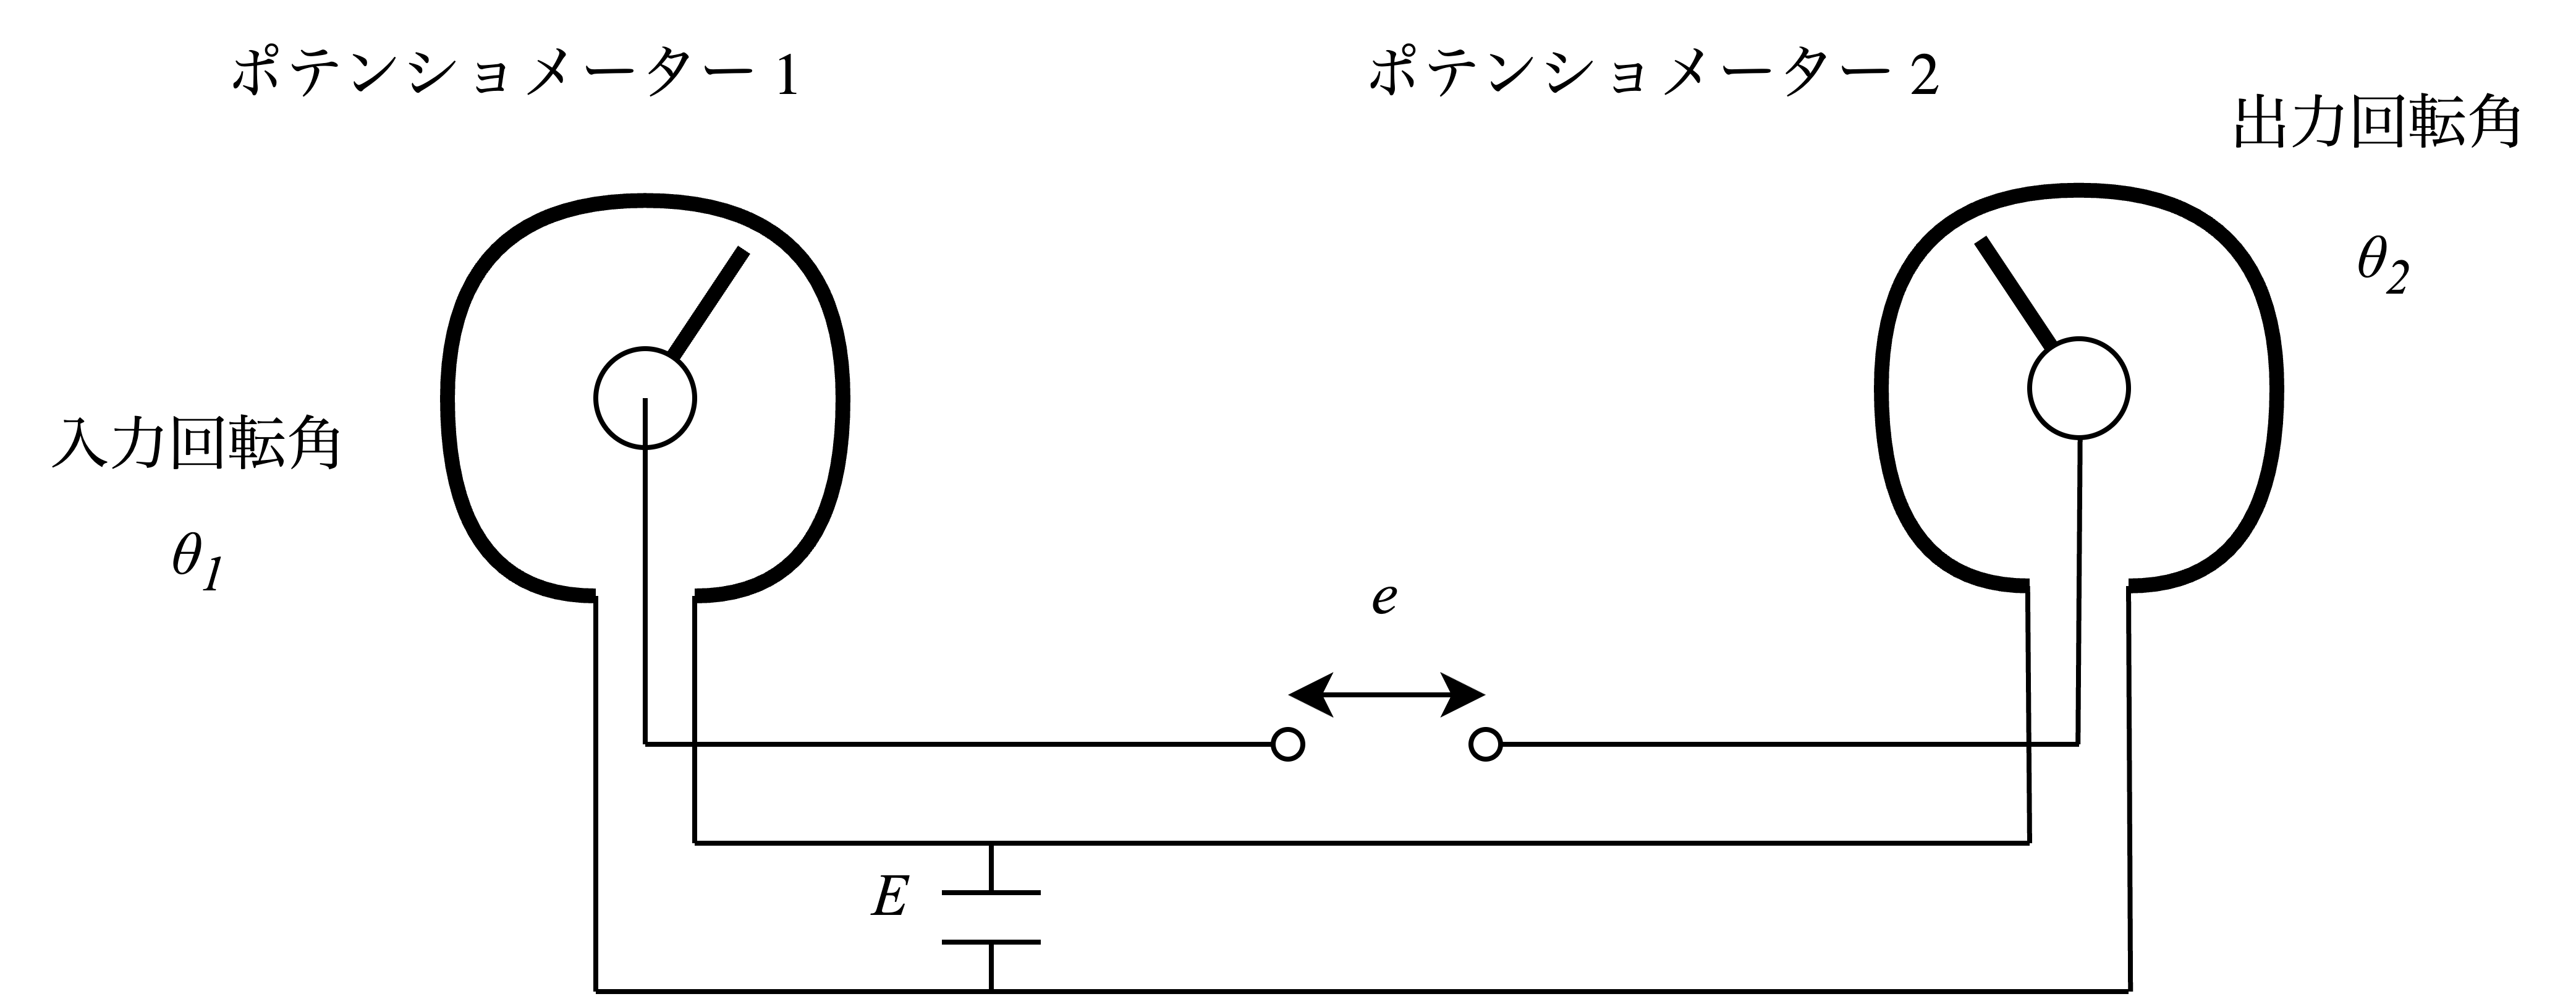
\includegraphics[width=0.8\linewidth]{src/figures/potentio-meter-2/potentio-meter-2.png}
    \caption{2台のポテンショメーターを用いた偏差検出回路}\label{fig:potentio-meter-detection}
\end{figure}


2台のポテンショメーターの印加電圧が異なる場合も、
\begin{equation}
    e = \dfrac{E_1}{\Theta} \theta_1 - \dfrac{E_2}{\Theta} \theta_2
\end{equation}
として得られる。
偏差電圧が0となってモーターが停止するときを考えると、
\begin{align*}
    e        & = 0                         \\
    \theta_2 & = \dfrac{E_1}{E_2} \theta_1
\end{align*}
のようになり、入力した所望角度の$E_1/E_2$倍だけ回転し停止することになる。

\subsection{サーボ増幅器}
サーボ増幅器は検出された微小な偏差電圧を増幅し、
サーボモーターを駆動するための電圧を生成する装置である。
一般には、積分や微分など系の特性を改善するために必要な信号処理などを行うが、
本実験では増幅のみを行う。
ブロック線図を図\ref{fig:amplifier}に示す。
\begin{figure}
    \centering
    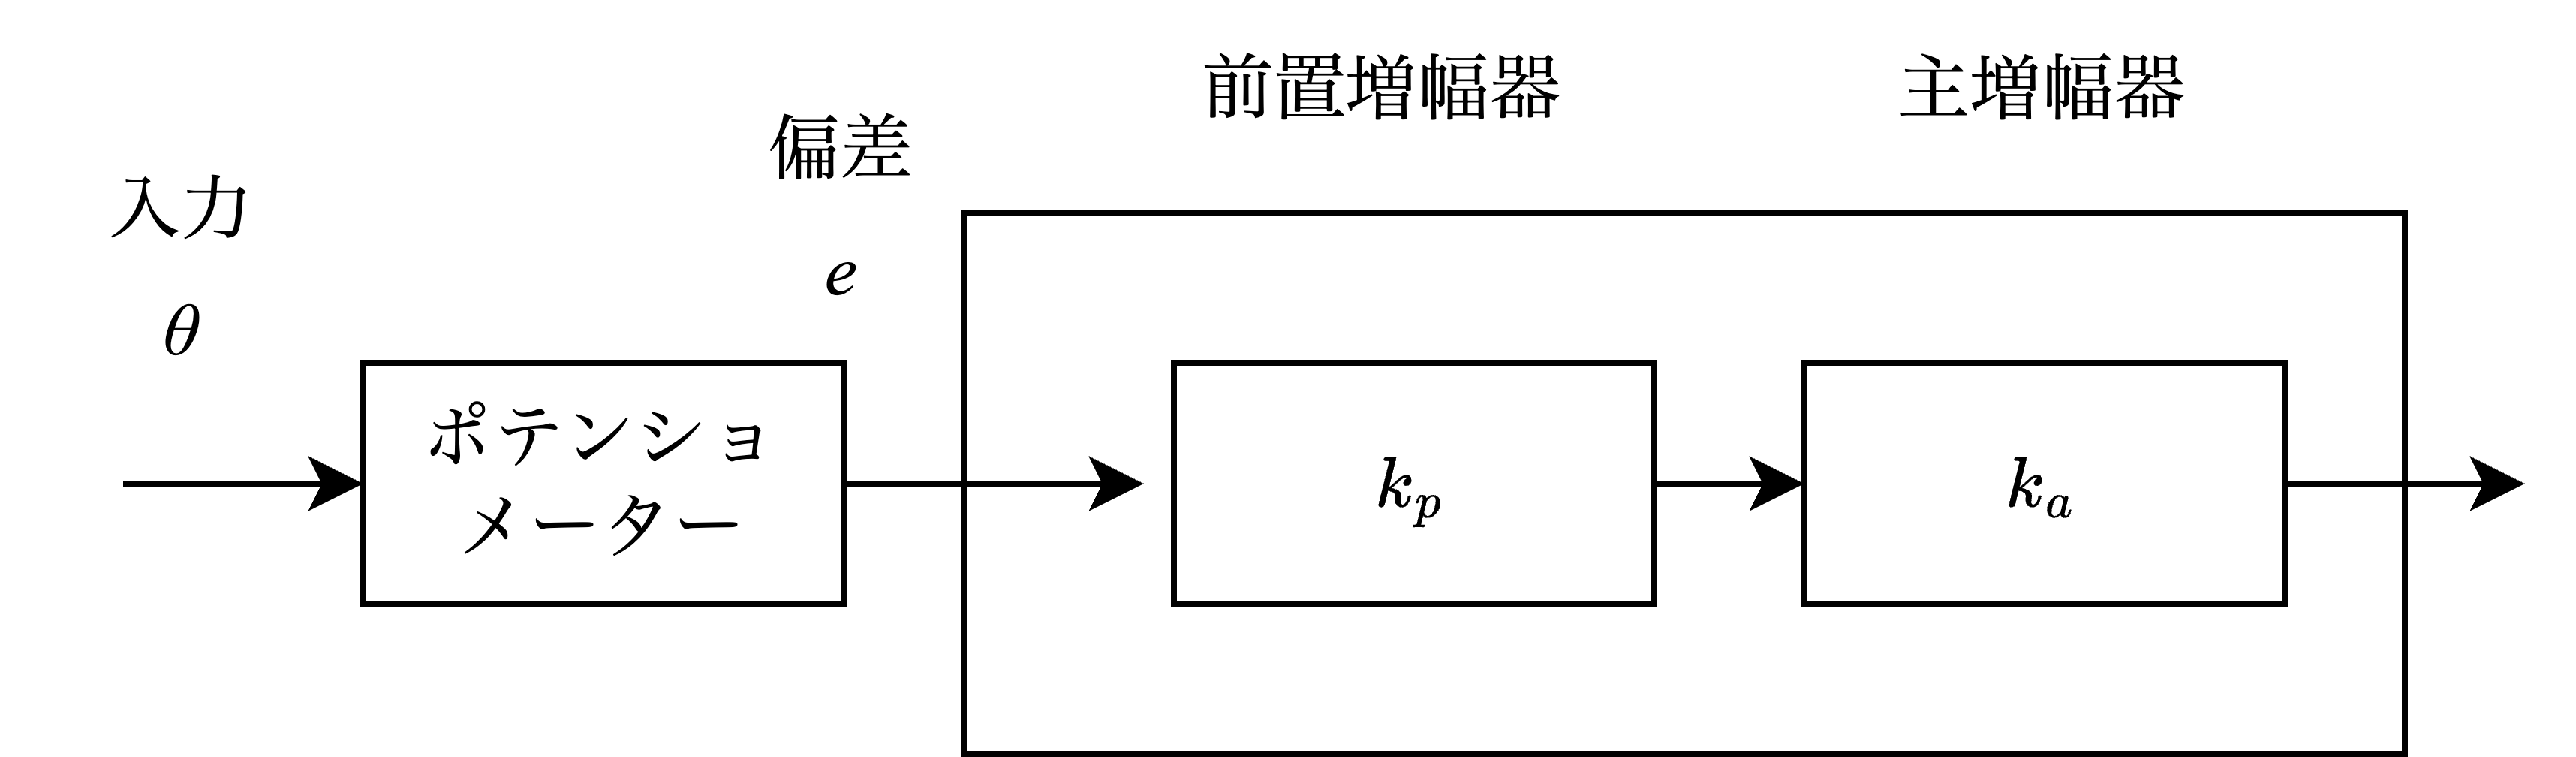
\includegraphics[width=0.8\linewidth]{src/figures/amplifier/amplifier.png}
    \caption{サーボ増幅器のブロック線図}\label{fig:amplifier}
\end{figure}


\subsection{サーボモーター}
本実験で用いるサーボモーターの特性関数を示す。
モーターの操作電圧を$e_c(t)$、モーターの回転速度を$\dot{\theta}(t)$とすると、
\begin{equation}
    T \odv{\dot{\theta}(t)}{t} + \dot{\theta}(t) = k_m e_c(t)
\end{equation}
これを各辺をLaplace変換して、
\begin{align}
    \left(TS + 1\right) \Theta(s) & = k_m E_c(s) \nonumber       \\
    \Theta(s)                     & = \dfrac{k_m}{TS + 1} E_c(s)
\end{align}
で、一次遅れ系となる。
ここで、ゲイン$k_m$、時定数$T$は次のように表される。
\begin{align*}
    k_m & = \dfrac{k_t}{R_a \left( D_m + \dfrac{k_t k_v}{R_a} \right)} \left( \approx \dfrac{1}{k_v} \right) \\
    T   & = \dfrac{J_m}{D_m + \dfrac{k_t k_v}{R_a}} \left( \approx \dfrac{J_m R_a}{k_t k_v} \right)
\end{align*}
但し、
\begin{align*}
    k_t & : \text{トルク定数}      \\
    k_v & : \text{速度定数}       \\
    R_a & : \text{電機子巻線抵抗}    \\
    J_m & : \text{電機子慣性モーメント} \\
    D_m & : \text{電機制動係数}
\end{align*}
である。
さらに、モーターの駆動する回転体物体が歯車比$n$の歯車列を介して
電機子軸に接続されているとき、
その負荷感性モーメントが$J_i$であるならば、
電機子軸に換算した全慣性モーメント
\begin{equation}
    J_{m}' = J_m + \dfrac{1}{n^2} J_i
\end{equation}
を$J_m$の代わりに用いる。
サーボ増幅器にサーボモーターを接続したブロック線図を
図\ref{fig:servo-motor}に示す。
\begin{figure}
    \centering
    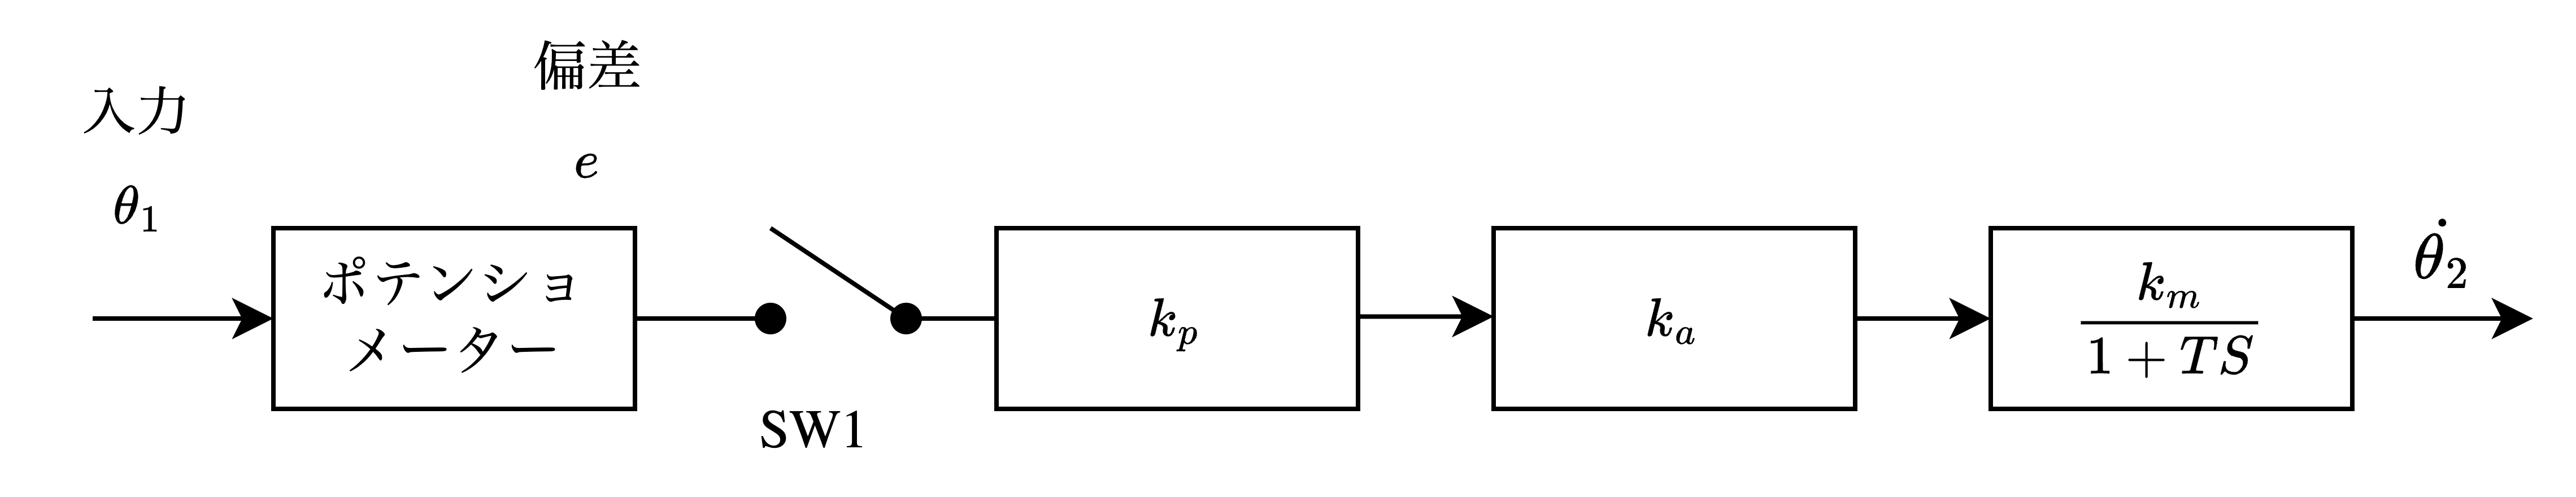
\includegraphics[width=0.8\linewidth]{src/figures/servo-motor/servo-motor.png}
    \caption{サーボ増幅器・サーボモーターのブロック線図}\label{fig:servo-motor}
\end{figure}


\subsection{フィードバック機構 / フィードバック補償 / P制御・PD制御}
図\ref{fig:servo-motor}までのブロック線図にフィードバック機構を加えると、
次の図\ref{fig:servo-block-line-detail}のようになる。
\begin{figure}
    \centering
    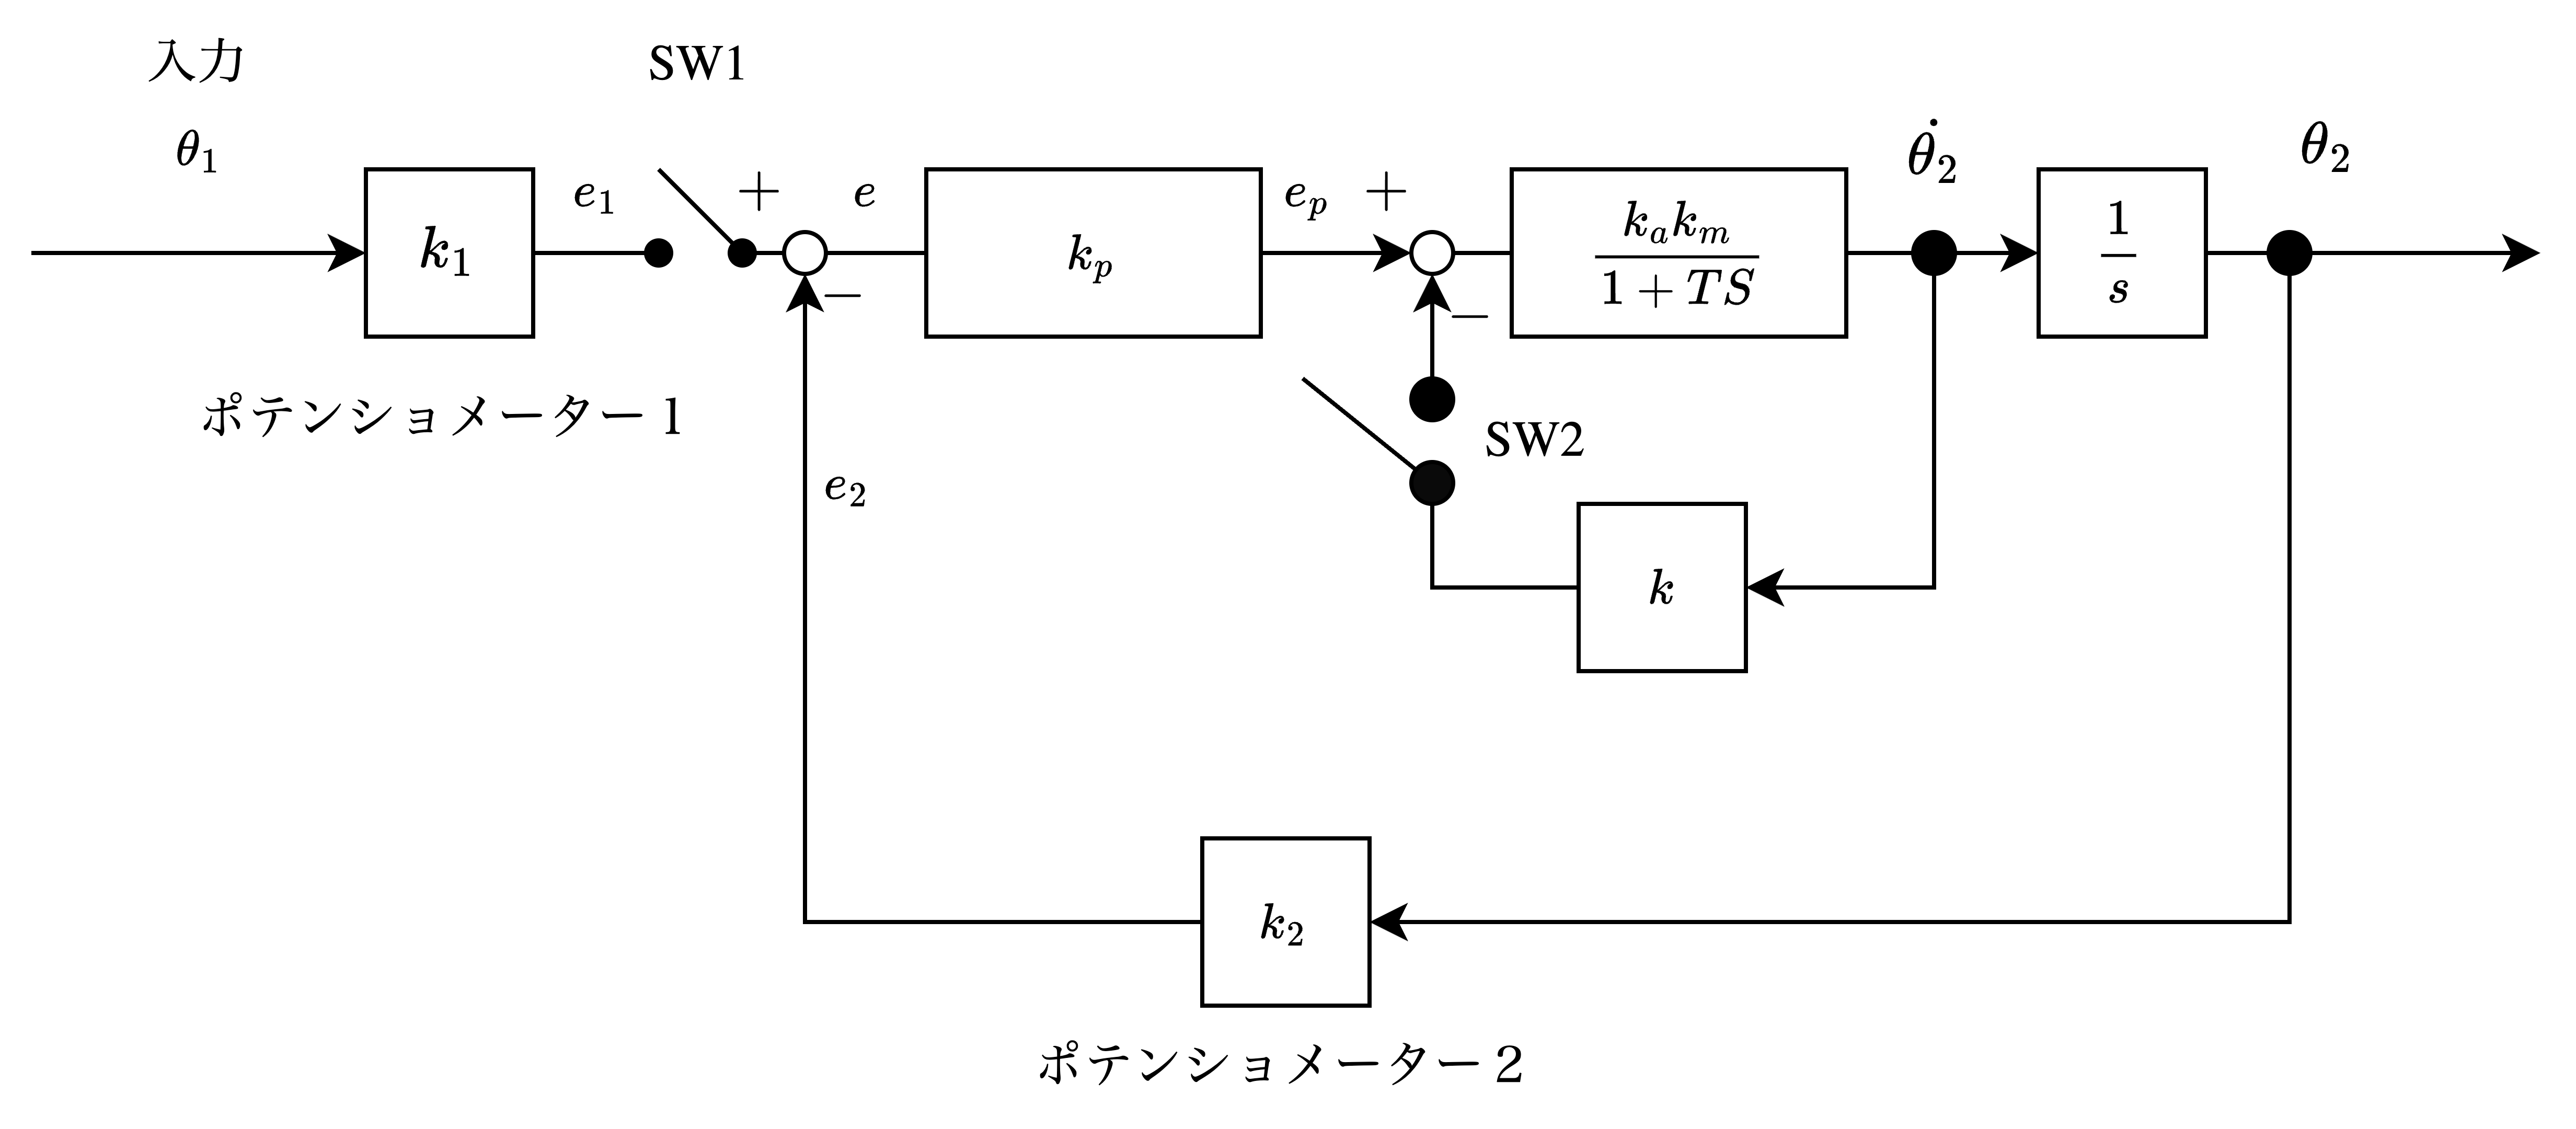
\includegraphics[width=0.8\linewidth]{src/figures/servo-block-line-detail/servo-block-line-detail.png}
    \caption{サーボ機構のブロック線図}\label{fig:servo-block-line-detail}
\end{figure}


SW2をOFFのとき、すなわち外側のフィードバックのみが働くときのサーボ機構全体での特性関数は、$K=k_a k_m$として、
\begin{align}
    \Theta_2                                                        & = \dfrac{1}{s} \dfrac{K}{1+TS} e_p \nonumber                                                   \\
                                                                    & = \dfrac{1}{s} \dfrac{K}{1+TS} k_p\left( k_1\Theta_1 - k_2 \Theta_2 \right) \nonumber          \\
    \left( 1 + \dfrac{1}{s}\dfrac{K k_p k_2}{1+TS} \right) \Theta_2 & = \dfrac{1}{s} \dfrac{K k_p k_1}{1+TS} \Theta_1 \nonumber                                      \\
    \Theta_2                                                        & = \dfrac{k_1}{k_2} \dfrac{K k_p k_2 / T}{s^2 + \dfrac{1}{T}s +\dfrac{K k_p k_2}{T}} \Theta_1 .
\end{align}
\begin{equation}\label{eq:characteristic-function-parameters}
    \begin{split}
        \omega & = \sqrt{\dfrac{K k_p k_2}{T}}    \\
        \zeta  & = \dfrac{1}{2\sqrt{K k_2 k_p T}}
    \end{split}
\end{equation}
として、
\begin{equation}\label{eq:characteristic-function}
    \Theta_2 = \dfrac{k_1}{k_2} \dfrac{\omega^2}{s^2 + 2\zeta\omega s + w^2} \Theta_1
\end{equation}
とかける。
ここで、$\omega$は固有振動数、$\zeta$は減衰係数と呼ばれる。
一般に$\zeta$は0.4~0.6程度が望ましいとされ、
$\omega$は速応性の目安で大きいほどよいとされる。
本実験では$K$、$k_2$、$T$は固定で変化できるのは$k_p$のみであるため、
$\omega$を大きく使用とすると、$\zeta$が小さくなりすぎるなどの問題が生じる。

そこで、SW2をONにし、内側のフィードバックも働かせたときの全体の特性関数は
\begin{align}\label{eq:characteristic-function2}
    \Theta_2                                                                       & = \dfrac{1}{s} \dfrac{K}{1+TS} \left(e_p - ks\Theta_2\right) \nonumber                     \\
    \left\{ 1 + \dfrac{1}{s}\dfrac{K}{1+TS}\left(k_pk_2+ks\right) \right\}\Theta_2 & = \dfrac{1}{s} \dfrac{K}{1+TS} k_p k_1 \Theta_1 \nonumber                                  \\
    \Theta_2                                                                       & = \dfrac{K k_p k_1 / T}{s^2 + \dfrac{1 + Kk}{T}s + \dfrac{Kk_p k_2}{T}} \Theta_1 \nonumber \\
    \Theta_2                                                                       & = \dfrac{k_1}{k_2} \dfrac{\omega^2}{s^2 + 2\zeta\omega s + \omega^2} \Theta_1
\end{align}
となり、
\begin{equation}\label{eq:characteristic-function2-parameters}
    \begin{split}
        \omega & = \sqrt{\dfrac{K k_p k_2}{T}}    \\
        \zeta  & = \dfrac{1+Kk}{2\sqrt{Kk_2k_pT}}
    \end{split}
\end{equation}
である。
\ref{eq:characteristic-function-parameters}式と異なり、
\ref{eq:characteristic-function2-parameters}式では
$\zeta$は$k$によって操作でき、$\omega$、$\zeta$をそれぞれ希望の値に近づけることができる様になった。
これをフィードバック補償といい、系全体の特性を向上させるために追加されるフィードバックである。

このSW2がOFFのとき、または$k=0$のときをP制御、$k>0$のときをPD制御とよぶ。


\end{document}
